\documentclass[a4paper, 11pt]{article}
\usepackage{geometry}
\geometry{letterpaper, margin=1in}
\usepackage{amsmath}
\usepackage{amssymb}  
\usepackage{amsthm}
\usepackage{ulem} 
\usepackage{graphicx}
\graphicspath{ {images/} }

\begin{document}
%Header-Make sure you update this information!!!!
\noindent
\large\textbf{Homework 2} \hfill \textbf{John Waczak} \\
\normalsize PH 431 \hfill  Date: \today \\
Prof. Bo Sun  \\
Worked with: Katy Chase, Daniel Still, Cassandra H. \\

\section*{1. Triangular Prism Dielectric}
\textit{Find the bound charge distribution} \\

\noindent Because $\mathbf{P} = P\hat{z}$ is uniform, we know that it will have zero divergence and thus $\rho_b = 0$. Therefore all of the bound charge must reside on the surface as $\sigma_b$. Let the bottom of the triangle be surface 1, then the top left is 2 and top right is 3. We can use the formula $\sigma_b = \mathbf{P} \cdot \hat{n}$ to find that: 
	\begin{equation*}
		\sigma_b = 
		\begin{cases}
			-P & \text{for surface 1} \\
			P/2 & \text{for surface 2 and 3}
		\end{cases}
	\end{equation*}
\noindent\textit{Find the total bound charge}\\

	
\noindent To find the total bound charge we need to integrate $\oint\limits_S \sigma_b ds$, so consider a small chunk of prism with length d. Then the area of each side of the prism is just $ad$ so that: 
	\begin{align*}
		Q_{b,\text{chunk}}&= -P(ad) + \frac{P}{2}(ad) + \frac{P}{2}(ad) \\ 
		&= 0
	\end{align*}
\noindent And since $Q_{b,\text{chunk}}=0$ regardless of our choice of d we can say $Q_b=0$. \\

\noindent\textit{What is the electric field produced by the prism at far field?}\\
 
In order to find the Electric field at far field, we need to find the potential at far field. For a regular dipole, the potential is given as: 
	\begin{equation*}
		\phi_{\text{dipole}} = \frac{1}{4\pi\epsilon_0}\frac{\mathbf{p}\cdot(\mathbf{r-r'})}{(|\mathbf{r-r'}|)^3}
	\end{equation*}
Where $\mathbf{p} = \mathbf{P}V$ for some volume. Consider then the dipole moment given by the volume in the prism shown below: \\
	\begin{center}
		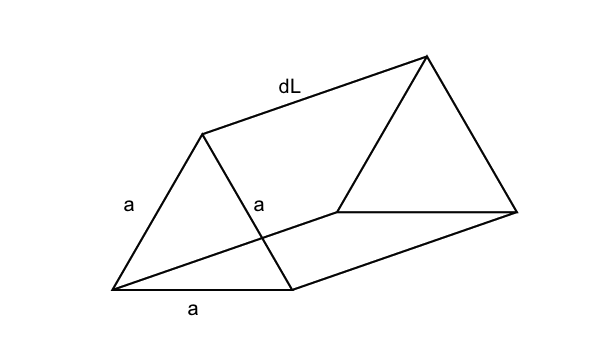
\includegraphics[scale=0.5]{prism}
	\end{center}
	
\noindent This has a dipole moment of $\mathbf{p} = P(A \cdot dl) \hat{z}$ where A is the area of the triangular cross section. So we can treat this as a single dipole at (0,0,0). Now if we want to find the potential for the infinitely long prism, we just need to let $dl = dy$ and integrate. Thus: 
	\begin{equation*}
		\phi_b = \frac{1}{4\pi\epsilon_0}\int\limits_{-\infty}^{\infty}\frac{(P(A \cdot dy) \hat{z})\cdot (\mathbf{r-r'})}{(|\mathbf{r-r'}|)^3}
	\end{equation*}

We can define the following: 
	\begin{align*}
		\mathbf{r'} &= y\hat{y} \\ 
		\mathbf{r} &= x\hat{x} + z\hat{z} \\ 
		\mathbf{r-r'} &= x\hat{x} -y\hat{y} + z\hat{z} \\ 
		|\mathbf{r-r'}| &= \sqrt{x^2+y^2+z^2}
	\end{align*}
Which we can say as we have modeled the prism as a simple dipole on the y axis. Thus the integration becomes: 
	\begin{align*}
		\phi_b &= \frac{1}{4\pi\epsilon_0}\int\limits_{-\infty}^{\infty}\frac{PAz}{(x^2+y^2+z^2)^{3/2}}dy \\
		&=\frac{PAz}{4\pi\epsilon_0}\frac{y}{(x^2+z^2)\sqrt{x^2+y^2+z^2}} \Bigg|_{y=-\infty}^{y=\infty} \\
		&=\frac{PAz}{4\pi\epsilon_0}\frac{2}{(x^2+z^2)}
	\end{align*}


Now if we are looking at the far field we have that $\frac{z}{(x^2+z^2)} \propto \frac{r}{r^2}=\frac{1}{r}$ so far away: 
	\begin{equation*}
		\phi_b = \frac{2PA}{4\pi\epsilon_0 r}
	\end{equation*}	
And thus the far field electric field $\mathbf{E_b}$ is: 
	\begin{align*}
		\mathbf{E}_b &= -\nabla\phi_b \\ 
		&= \frac{2PA}{4\pi\epsilon_0 r^2}\hat{r}
	\end{align*}	
In terms of the area of the face of the prism that is: 
	\begin{equation*}
		\mathbf{E}_b = \frac{\sqrt{3}a^2}{4}\frac{2P}{4\pi\epsilon_0 r^2}\hat{r} = \frac{\sqrt{3}a^2P}{8\pi\epsilon_0 r^2}\hat{r}
	\end{equation*}
	
\section*{2. Dielectric sphere in a second dielectric}
\textit{Solve for the electric field inside and outside the sphere}\\

\noindent To solve this problem, I will first identify the necessary boundary conditions that will allow us to uniquely solve Laplace's equation for the electric field inside the sphere and outside. Let R denote the radius of the sphere. We have that: 
	\begin{align}
		\phi_{in}(r=R, \theta) &= \phi_{out}(r=R, \theta) \\ 
		\epsilon_1 \frac{\partial \phi_{in}}{\partial r} &= \epsilon_2 \frac{\partial \phi_{out}}{\partial r} \\ 
		\phi_{out}(r>>R) &= \phi_ext = -E_0z = -E_0r\cos(\theta)
	\end{align}

\noindent The first condition (1) comes from the required continuity of the potential. The second follows directly from the fact that the displacement field is proportional to the Electric field and must have a continuous perpendicular element (in $\hat{r}$ direction) across the interface. The third condition dictates that at far field, the electric field should decay to be that of just the external field that is polarizing the dielectrics. \\

\noindent From the azimuthal symmetry we can immediately determine the form for $\phi_{in}$ and $\phi_{out}$ in terms of Legendre polynomials: 
	\begin{align*}
		\phi_{in}(r,\theta) &= \sum\limits_{l=0}^{\infty}A_l r^l P_l(\cos(\theta)) \\
		\phi_{out}(r, \theta) &= -E_0r\cos(\theta) + \sum\limits_{l=0}^{\infty}\frac{B_l}{r^{l+1}}P_l(\cos(\theta))
	\end{align*}
	
Now we can apply the boundary conditions to these equations. Looking at (1) at we get: 
	\begin{equation*}
	\begin{cases}
		A_lR^l = \frac{B_l}{R^{l+1}} & l\neq 1 \\
		A_1R = -E_0R + \frac{B_1}{R^2} & l = 1 
	\end{cases}
	\end{equation*}
	
Note that $P_1(\cos(\theta))= \cos(\theta)$. (2) tells us to differentiate the equations with respect to r. Thus: 
	\begin{equation*}
	\begin{cases}
		\frac{\epsilon_1}{\epsilon_2}A_llR^{l-1} = \frac{-(l+1)B_l}{R^{l+2}} & l\neq 1 \\ 
		\frac{\epsilon_1}{\epsilon_2}A_1R = -E_0-\frac{2B_1}{R^3} & l=1
	\end{cases}
	\end{equation*}

Using the first $l\neq1$ case we will show that $A_l=B_l=0$.
	\begin{align*}
		A_l &= \frac{B_l}{R^{2l+1}} \\
		\frac{\epsilon_1}{\epsilon_2}\Big(\frac{B_l}{R^{2l+1}}\Big)lR^{l-1} &= \frac{-(l+1)B_l}{R^{l+2}} \\ 
		\frac{\epsilon_1}{\epsilon_2}\Big(\frac{B_l}{R^{2l+1}}\Big)lR^{2l+1} &= -(l+1)B_l \\ 
		\frac{\epsilon_1}{\epsilon_2}B_ll &= -(l+1)B_l \\ 	
		\Rightarrow B_l &= 0 \Rightarrow A_l = 0	
	\end{align*}
Thus all we need to worry about is $l=1$. Repeating the same process for the other set of equations we have: 
	\begin{align*}
		A_1 &= -E_0+\frac{B_1}{R^3} \\ 
		\frac{\epsilon_1}{\epsilon_2}[-E_0 \frac{B_1}{R^3}] &= -E_0 -2\frac{2B_1}{R^3} \\ 
		-E_0\frac{\epsilon_1}{\epsilon_2}+\frac{B_1}{R^3}\frac{\epsilon_1}{\epsilon_2}& =-E_0-2\frac{B_1}{R^3} \\
		\frac{B_1(\frac{\epsilon_1}{\epsilon_2}+2)}{R^3} &= E_0\Big(\frac{\epsilon_1}{\epsilon_2}-1\Big) \\
		B_1 &= \frac{R^3E_0(\frac{\epsilon_1}{\epsilon_2}-1)}{(\frac{\epsilon_1}{\epsilon_2}+2)} \\
		A_1 &= -E_0 + \frac{E_0(\frac{\epsilon_1}{\epsilon_2}-1)}{(\frac{\epsilon_1}{\epsilon_2}+2)}
	\end{align*}
So now we have a set of equations that satisfies the necessary boundary equations and Laplace's equation. 
	\begin{align}
		\phi_{in}(r\leq R, \theta) &= -\frac{3E_0}{\frac{\epsilon_1}{\epsilon_2}+2}r\cos(\theta)\\
		\phi_{out}(r\geq R, \theta) &= \frac{(\frac{\epsilon_1}{\epsilon_2}-1)}{(\frac{\epsilon_1}{\epsilon_2}+2)}R^3E_0\frac{cos(\theta)}{r^2}-E_0r\cos(\theta)
	\end{align}	
Now to find the electric fields we will simply take the spherical gradient of these functions using mathematica. This gives: 
	\begin{align*}
		\mathbf{E_{in}} &=  \frac{3\cos(\theta)E_0}{2+\frac{\epsilon_1}{\epsilon_2}} \hat{r} + \frac{-3\sin(\theta)E_0}{2+\frac{\epsilon_1}{\epsilon_2}} \hat{\theta}   \\
		\mathbf{E_{out}} &= \Bigg(E_0\cos(\theta)+\frac{2\cos(\theta)(\frac{\epsilon_1}{\epsilon_2}-1)}{r^3(2+\frac{\epsilon_1}{\epsilon_2})} \Bigg) \hat{r} + 
		 \Bigg(\frac{-E_0\sin(\theta)\cdot((r^3-R^3)\epsilon_1+(2r^3+R^3)\epsilon_2)}{r^3(\epsilon_1+2\epsilon_2)} \Bigg) \hat{\theta}\\ 
	\end{align*}	
It is worth noting that if we instead find the Cartesian gradient of $\phi_{in}$ we get: 
	\begin{equation}
		\mathbf{E}_{in} = \frac{3zE_0}{2+\frac{\epsilon_1}{\epsilon_2}}\hat{z}
	\end{equation}	
Which is uniform in the z direction as we expect!\\

\noindent\textit{What is the charge density at the interface?}\\

\noindent To find the charge density at the interface we can apply Gauss's law using a very thin cylinder such that there is no flux from the $E_{\theta}$ component of the fields, only the radial, i.e.: 
	\begin{align*}
		\int\limits_S \mathbf{E}\cdot d\mathbf{s} &= \frac{1}{\epsilon_0}\int\limits_S \sigma ds\\
		E_{out}A-E_{in}A &= \frac{\sigma A}{\epsilon_0 A}
	\end{align*}
Where A is the area of the face of the cylinder. Therefore we have that: 
	\begin{equation*}
		\sigma = \epsilon_0 \Delta E(r=R)
	\end{equation*}
Using our equations for $E_{in}$ and $E_{out}$ we have that: 
	\begin{equation}
		\sigma = \epsilon_0 \Bigg( \frac{3\cos(\theta)E_0(\epsilon_1-\epsilon_2)}{\epsilon_1+2\epsilon_2}\Bigg)
	\end{equation}
\noindent\textit{Prove that $\mathbf{E}_{\theta}$ is continuous across the interface.} \\

\noindent To show this all we need to do is set the theta components of $E_{in}$ and $E_{out}$ equal at $r=R$. 
	\begin{align*}
		 \frac{-3\sin(\theta)E_0}{2+\frac{\epsilon_1}{\epsilon_2}} &=\Bigg(\frac{-E_0\sin(\theta)\cdot((R^3-R^3)\epsilon_1+(2R^3+R^3)\epsilon_2)}{R^3(\epsilon_1+2\epsilon_2)} \Bigg) \\
		 &= \frac{-3\sin(\theta)E_0\epsilon_2}{\epsilon_1+2\epsilon_2}\\
		 &= \frac{-3\sin(\theta)E_0}{2+\frac{\epsilon_1}{\epsilon_2}}
	\end{align*}
Thus we have that $E_{\theta}$ is continuous at the boundary. \\

\noindent\textit{What is the drop in $D_{\theta}$ across the interface?} \\ 

\noindent In the dielectric we have that $\textbf{D}/\epsilon = \textbf{E}$. Thus we know that there will be discontinuities in $D_{\theta}$ if $E_{\theta}$ is continuous because the same condition in terms of displacement fields reads: 
	\begin{equation*}
		\epsilon_1 \mathbf{D_{\theta,\text{in}}} = \epsilon_2 \mathbf{D_{\theta,\text{out}}}
	\end{equation*}
Therefore we can define the difference as: 
	\begin{align*}
		\Delta \mathbf{D_{\theta}} &= \Delta\mathbf{E_{\theta}}(r=R)\cdot(\epsilon_2-\epsilon_1) \\
		&=\frac{-3\sin(\theta)E_0}{2+\frac{\epsilon_1}{\epsilon_2}}(\epsilon_2-\epsilon_1)
	\end{align*}
	
	
\section*{Mathematica Code}
\includegraphics[scale=1.0]{code}
\end{document}


















